\documentclass[a4paper,11pt]{article}

\input ../include/preamble.tex

\usepackage{tikz}
\usetikzlibrary{automata,arrows,topaths,calc,positioning}

\usepackage{subcaption}

\usepackage{changepage}

\usepackage{listings}

\lstdefinelanguage{elixir}{
	morekeywords={case,catch,def,do,else,false,%
		use,alias,receive,timeout,defmacro,defp,%
		for,if,import,defmodule,defprotocol,%
		nil,defmacrop,defoverridable,defimpl,%
		super,fn,raise,true,try,end,with,%
		unless},
	otherkeywords={<-,->},
	sensitive=true,
	morecomment=[l]{\#},
	morecomment=[n]{/*}{*/},
	morestring=[b]",
	morestring=[b]',
	morestring=[b]"""
}

\lstset{language=elixir}

\begin{document}

\title{
    \textbf{A MIPS emulator}\\
    \large{Programming II}
}
\author{Johan Montelius}
\date{Spring Term 2021}
\maketitle
\defaultpagestyle

\section*{Introduction}

In this exercise we will combine your knowledge of computer
architecture and concurrent programming to implement an emulator of a
simple MIPS processor. You should have basic understanding of the
architecture and how the data path is implemented. We will only
implement a small subset of the MIPS machine instructions but it will
be possible to extend it.

\section{MIPS}

There are of course many different ways a MIPS cpu can be designed but
we will follow the description given in chapter four of ``Computer Organization and
Design'' by Patterson and Hennessy. If you have not studied their
desciption you should do so before starting with the implementation,
this is not a turiorial of the MIPS architecture.

\subsection{high-level design}

We will divide the processor into five unitss, each unit will be
implemented as an Elexir process and the data-paths will be Elixir
messages. This might not be a straight forward way to implement an
emulator but it more challenging and you will learn a lot about concurrency in Elixir.

The units, which will also be Elixir modules, are:

\begin{itemize}

\item {\bf Instruction} : instruction fetcher, will retrieve the next
  instruction, divide it into its parts and send them to other units.

\item {\bf Register} : register unit, reads the contents of the registers
  and passes the vakues to the ALU.

\item {\bf ALU} : performs the arithmetic operations and passes the result to the memory unit.

\item {\bf Memory} : handles load and store operation and in the case
  of a store passes the read value to the register unit.

\item {\bf Next} : the unit that will decide which instruction to
  execute next. In the begining this is simlpy the next instruction
  but when we introduce branch and jump instructions this unit will
  have more things to do.

\item {\bf Controller} : the brain of the CPU, will receive the op
  codes from the instruction unit and direct the other units what to do.
  
\end{itemize}

In Fig.\ref{fig:flow} we see an overview of the CPU with the primary
data flow. We have all units but the controll unit to simplify the
image. The Instruction unit will fetch the next instruction and send the
register identifiers to the Register unit. It will also send a
possible immediate value directly to the ALU and an incremented
program counter to the Next unit.

The Register unit will send the content of the regiterst to the ALU
unit but also pass one value directly to the memory unit.  This will
typiclaly be a value that should be stored. The ALU does its
computation and sends the result, and address, to the memory unit. It
will also send a message to the Next unit describing the outcome of
the operation i.e. if it was zero or not.

The memory unit will, if it is a load instruction that is executed,
send the retrieed value back to the register unit. The register unit
will then stor it in one of the registers.

The Next unit will recieve both the incremented progroam counter from
the Instruction unit and a value form the Register unit. Depending on the
instruction, and the outcome of teh ALU operation, the next code
address is selected and sen to the Instruction unit.


\begin{figure}
  \centering 
  \begin{tikzpicture}[unit/.style={rectangle, very thick, minimum height=1cm, minimum width=2cm, text centered}]

%Nodes
\node[unit]    (instr)                      {Instruction};
\node[unit]    (reg)       [right=of instr] {Register};
\node[unit]    (alu)       [right=of reg]   {ALU};
\node[unit]    (mem)       [right=of alu]   {Memory};
\node[unit]    (nxt)       [above=of alu]   {Next};

%Lines 
\draw[->] (instr.east) -- (reg.west);
\draw[->] (reg.east) -- (alu.west);
\draw[->] (alu.east) -- (mem.west);
\draw[->] (alu.north) -- (nxt.south);
\draw[->] (instr.north) .. controls +(up:1cm) and +(left:1cm) .. (nxt.west);
\draw[->] (instr.south) .. controls +(down:1cm) and +(down:1cm) .. (alu.south);

\draw[->] (reg.south) .. controls +(down:1cm) and +(down:1cm) .. (mem.south);
\draw[->] (nxt.north) .. controls +(up:2cm) and +(left:3cm) .. (instr.west);
\draw[->] (mem.north) .. controls +(up:1cm) and +(up:1cm) .. (reg.north);

  \end{tikzpicture}
  \caption{The data flow of the processor.} \label{fig:flow}
\end{figure}

What each unit shoudl do is of course determined by the Controller
unit that is given the op code from the Instruction unit. The controller is
normally described as two units, one main controller and a separate
ALU controller. We will combine these into one unit; nothing is gained
by separating them.


\subsection{signals}

When you see the regular description of the CPU architecture you will
see how for example the Instruction unit sends three different signals to
the Register unit: read 1, read 2 and write register. We will
implement this in one message. The register unit will in the same way
pass two values to the ALU i one message.  Our implementation is thus
more focused on which information that is passed between the units
rather than how this would realized in a hardware implementation.

\subsection{the memory}

We will make things a bit easier by separating the code from the main
memory. In real life, the code is of course in the main memory but it
makes things easier if we keep them in two different data
structures. The only limitations that this will mean is that 1/ we
will not be able to change the code during execution and 2/ we can not
use the program counter as a base address when accessing data.

The first limitation is something we can live with, few programs write
to the code segment anyway. The second limation could be a problem but
not in the MIPS architecture. The only instructions that operate
relative to the program counter is the branch and jump
instructions. These instruction do not read from the main memory bu
only change the program counter and we will be able to handle this.

Since we will not write to the code area we can implement this with a
data structure that maximize read performance. The memory should be
some data structure with efficient random read and write operations.


\subsection{the controller}

The Controller is of course the heart of teh system. It will receive
one message from the Instruction unit with teh op code and ALU function
code. It then determines what the different units should do and sends
the correspondng signals. These are the signals:

\begin{itemize}

\item {\bf Register} : the Register unit can proceed and send the two
  values to the ALU but must then know if it should store the value
  returned from the Memory unit and which register to store it in.

\item {\bf ALU} : the ALU must of course know which operation to
  perform but it must also know it it should use both values from the
  Register unit or if it should use the immediate value from the Instruction unit.

\item {\bf Memory} : the Memory unit must know if it should perform a
  load, stor or no-op. If it is a load instrucktion the read value
  should be returned to the Register unit. If it is a store operation
  it does not matter what it outputs (but it must send a value)
  otherwise it sends the value it received from the ALU.

\item {\bf Next} : the Next unit needs to know if the operation is a
  branch or jump instruction in order to determine how to select the
  next program counter.
  
\end{itemize}

\subsection{asynchronous pipeline}

One thing that we have not mentioned is how to time things, where is
the clock pulse and when should units proceed. The answer is that the
design is asynchronous and a unit can proceed as soon as it has the
available information.

Asynchronous does not mean chaos so we need to think about how this
should work. One example where things could go wrong is if the Next
unit decides to send the next program counter to the Instruction unit
since it knows it's not a branch instruction being executed - why wait
for the ALU if the zero information is not needed? The problem is if
the next instruction is a branch instruction and the zero messge from
the previous instructions is read. We need a way to keep things
synchronized even though messages are sent asynchrounous. 

To make this work we first of all rely on the ordered delivery of
messages. What ever happen, messages will not be delivered out of
order. Elixir does of course not guarantee that messages do arrive but
this is something that we will ignore, we work under the assumption
that all messages do arrive (which they will if we do not distribute
the system over a network).

To visualize the communication protocol we draw a sequence diagram.

\begin{figure}
  \centering 
  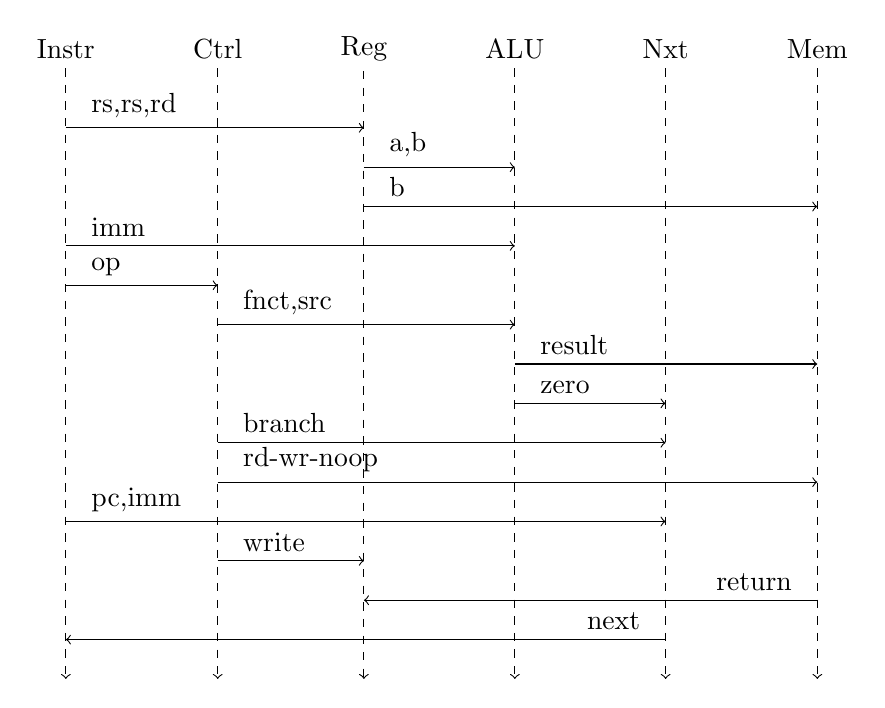
\begin{tikzpicture}
    \node[]                 (instr) {Instr};
    \node[right = of instr] (ctrl)  {Ctrl};
    \node[right = of ctrl]  (reg)   {Reg};
    \node[right = of reg]  (alu)   {ALU};    
    \node[right = of alu]   (nxt)   {Nxt};
    \node[right = of nxt]   (mem)   {Mem};    
    
    
    \draw[->, dashed] (instr) -- ($ (instr) - (0,8)$);
    \draw[->, dashed] (reg) -- ($ (reg) - (0,8)$);
    \draw[->, dashed] (ctrl) -- ($ (ctrl) - (0,8)$);
    \draw[->, dashed] (alu) -- ($ (alu) - (0,8)$);
    \draw[->, dashed] (nxt) -- ($ (nxt) - (0,8)$);    
    \draw[->, dashed] (mem) -- ($ (mem) - (0,8)$);    
    
    \draw[->] ($(instr) - (0,1)$) node[xshift=0.2cm, anchor= south west]{rs,rs,rd} --  ($(reg)  - (0,1)$);

    \draw[->] ($(reg) - (0,1.5)$) node[xshift=0.2cm, anchor= south west]{a,b} --  ($(alu)  - (0,1.5)$);

    \draw[->] ($(reg) - (0,2.0)$) node[xshift=0.2cm, anchor= south west]{b} --  ($(mem)  - (0,2.0)$);
    

    \draw[->] ($(instr) - (0,2.5)$) node[xshift=0.2cm, anchor= south west]{imm} --  ($(alu)  - (0,2.5)$);

    \draw[->] ($(instr) - (0,3.0)$) node[xshift=0.2cm, anchor= south west]{op}  --   ($(ctrl)  - (0,3.0)$);

    \draw[->] ($(ctrl) - (0,3.5)$) node[xshift=0.2cm, anchor= south west]{fnct,src} --  ($(alu)  - (0,3.5)$);    

    \draw[->] ($(alu) - (0,4.0)$) node[xshift=0.2cm, anchor= south west]{result} --  ($(mem)  - (0,4.0)$);

    \draw[->] ($(alu) - (0,4.5)$) node[xshift=0.2cm, anchor= south west]{zero} --  ($(nxt)  - (0,4.5)$);    

    \draw[->] ($(ctrl) - (0,5.0)$) node[xshift=0.2cm, anchor= south west]{branch} --  ($(nxt)  - (0,5.0)$);

    \draw[->] ($(ctrl) - (0,5.5)$) node[xshift=0.2cm, anchor= south west]{rd-wr-noop} --  ($(mem)  - (0,5.5)$);    

    \draw[->] ($(instr) - (0,6.0)$) node[xshift=0.2cm, anchor= south west]{pc,imm} --  ($(nxt)  - (0,6.0)$);    
    
    \draw[->] ($(ctrl) - (0,6.5)$) node[xshift=0.2cm, anchor= south west]{write}  -- ($(reg)  - (0,6.5)$);    

    \draw[->] ($(mem) - (0,7.0)$) node[xshift=-0.2cm, anchor= south east]{return}  -- ($(reg)  - (0,7.0)$);

    \draw[->] ($(nxt) - (0,7.5)$) node[xshift=-0.2cm, anchor= south east]{next}  -- ($(instr)  - (0,7.5)$);            
    
  \end{tikzpicture}
  \caption{The network protocoll of the CPU.} \label{fig:seq}
\end{figure}



So now when we have the over all undestanding of the emulator let's do
some coding.



\section{The implementation}






\end{document}

